\chapter{System Design And Architecture}
\section{System architecture}
%Begin from here





\section{Multimedia database design}
%Begin from here
\subsection{The purpose of our data base}
The puspose of our data base is to work as images and videos search engine server.This is achieved by storing images and videos with 
their pre computed extracted features then takes a an image or video as input form the user and query the data base storge based on 
the extracted features of the input material and outputs the most relevant matrial to the input model.
\vskip 0.2in
The project database supports three filter techniques for images retreival operation which are mean color, histogram, and color layout and 
one technique for video retreival operation base on histogram of the key frames.
\subsection{Required information}
To achieve the required techniques, we need our database to hold some information about each stored element.
\begin{enumerate}
    \item Images features
    \begin{itemize}
        \item We store the mean color value for each image. Mean color is calculated by finding the average of the pixels values for each channle separatley,
        then finding the averge between the three values resulting from each channel.        
        \item Histogram information is needed to be stored,but if we store the whole 255 values of each histogram ,we will consume huge amount of storage.
        The solution we have used is to divide the histogram into five regions and get the averge of each region so we convert the 255 values into 5 values only and store them in the database.
        we need these five values for only first step in filtering and then we compare using the complete histogram -255 values- for the filtered images.
    \end{itemize}
    \item Video features
    \begin{itemize}
        \item Instead of storing the whole video frames we only store the information about the key frames of the video. Each key frame is related to its video through
        "ID", then we deal with key frames in the same manner of the images so we store five values for the histogram of each key frame.
    \end{itemize}
\end{enumerate}

\subsection{Database Schema}
The data base consists of three main tables :
\begin{itemize}
    \item The first tables is "Image" which holds the information for each image.        
    \item The second is "Video" which holds only the ID and Path of each video.
    \item The third table is "Key Frame".
    this table holds all the key frames of all stored videos and relate each key fram to its video using the video ID.
\end{itemize}
\vskip 0.2in

\begin{figure}[H]
    \centering
    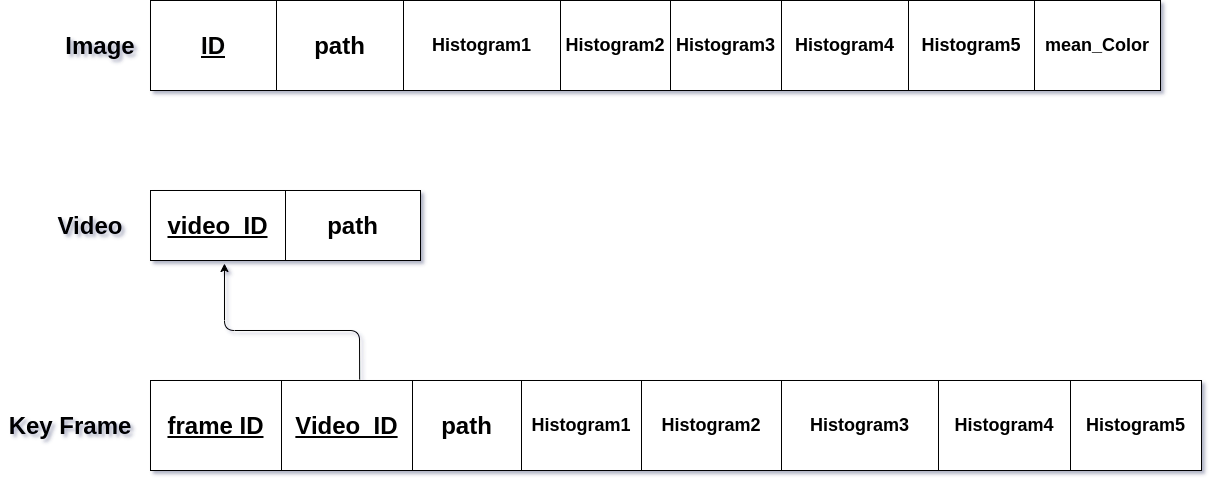
\includegraphics[width=120mm,height=70mm]{Images/database.png}
    \caption{Data base schema}
  \end{figure}
\subsection{Primary keys and foriegn keys}
\begin{itemize}
    \item Primary keys of each table are:
    \begin{enumerate}
        \item Image table Primary key is the Id of each image.      
        \item Video table Primary key is the Id of each video.
        \item Key frame table Primary key is a composite key from the id of each key frame and the id of the refered video.  
    \end{enumerate}        
    \item Foriegn keys used are:
    \begin{itemize}
        \item Key frame table has the referenced video id as a foriegn key which relates each key frame to its original video.      
    \end{itemize}
\end{itemize}

\section{System design}
%Begin from here





\section{Testing scenarios and results}
%Begin from here
